\documentclass[twocolumn]{aastex62}

% typography
\usepackage[T1]{fontenc}

\setlength{\parindent}{1.\baselineskip}
\newcommand{\acronym}[1]{{\small{#1}}}
\newcommand{\package}[1]{\textsl{#1}}
\newcommand{\gaia}{\textsl{Gaia}}

% aastex parameters
% \received{not yet; THIS IS A DRAFT}
%\revised{not yet}
%\accepted{not yet}
% % Adds "Submitted to " the arguement.
% \submitjournal{ApJ}
\shorttitle{the jhelum puzzle}
\shortauthors{bonaca et al.}

%@arxiver{}
\usepackage{amsmath}

\begin{document}\sloppy\sloppypar\raggedbottom\frenchspacing % trust me

\title{Multiple components of the Jhelum stellar stream}

\correspondingauthor{Ana Bonaca}
\email{ana.bonaca@cfa.harvard.edu}

\author[0000-0002-7846-9787]{Ana Bonaca}
\affil{Center for Astrophysics | Harvard \& Smithsonian, 60 Garden St, Cambridge, MA 02138, USA}

\author[0000-0002-1590-8551]{Charlie Conroy}
\affil{Center for Astrophysics | Harvard \& Smithsonian, 60 Garden St, Cambridge, MA 02138, USA}
% \affil{Harvard--Smithsonian Center for Astrophysics, 60 Garden St, Cambridge, MA 02138, USA}

\author{collaborators}

% \author[0000-0003-2866-9403]{David W. Hogg}
% \affiliation{Center for Cosmology and Particle Physics,
% Department of Physics,
% New York University}
% \affiliation{Center for Data Science,
% New York University}
% \affiliation{Max-Planck-Institut f\"ur Astronomie, Heidelberg}
% \affiliation{Flatiron Institute, Simons Foundation}

% David, Adrian, Josh
%% Kathryn

\begin{abstract}\noindent % trust me
Tidally disrupted globular clusters produce long, thin and dynamically cold stellar streams that preserve a historical record of any gravitational perturbations.
Signatures of perturbation appear as low surface brightness features and have historically been hard to detect due to contamination from field stars.
We use astrometric data from the Gaia second data release and photometry from the Dark Energy Survey to identify highly probable members of Jhelum, a retrograde stellar stream in the Milky Way halo.
The decontaminated map of Jhelum reveals that the stream has two components: a thin component and an offset, diffuse component.
The width and the significance of the diffuse component vary along the stream, however, the two components have the same ratio of blue straggler to blue horizontal branch stars.
This suggests that the debris originates from a single progenitor, and that the complex morphology has been imparted by its dynamical evolution in an evolving environment.
% Further modeling of Jhelum, as well as similar studies of other streams, should .
\end{abstract}

\keywords{%
stars:~kinematics~and~dynamics
  ---
Galaxy:~halo
  ---
Galaxy:~kinematics~and~dynamics
}

\section{Introduction}
\label{sec:intro}

% - mw provides opportunity to study processes of gal formation in archaelogical evidence
% - halo dynamical times, streams track that change
% 
% - streams regular so far
% - dynamical environment, should have features
% - now with gaia can study those

Stars escaping from globular clusters form thin, dynamically cold tidal streams \citep[e.g.,][]{combes1999}.
The phase-space distribution of tidal debris is predominantly determined by the gravitational tidal field, so \citet{johnston1999} proposed measuring the distribution of matter in the Galaxy using stellar streams.
In detail, the mean track of a stream constrains the enclosed mass at its current location \citep{bh2018}.
As more than 40 stellar streams have been discovered at a range of distances in the Milky Way halo \citep[see][for a recent review]{gc2016}, streams should provide a three-dimensional map of the Galaxy.

Being long and thin structures, stellar streams also preserve a historical record of gravitational perturbations on small scales and have been discussed as tracers of dark matter substructure \citep[e.g.,][]{johnston2002, carlberg2009}.
A telltale signature of an interaction with a dark matter subhalo is a gap in the stellar density along the stream \citep[e.g.,][]{yoon2011, eb2015}.
Tantalizing hints of stream gaps were first observed in the early photometric surveys \citep[e.g.,][]{carlberg2012,cg2013}, and gaps were definitively detected in the GD-1 stellar stream \citep{gd2006} when \citet{pwb} used \gaia\ proper motions to cleanly select likely stream members.
This discovery opened a new era in which globular cluster streams are no longer simple tracers of the global gravitational potential, but instead provide additional constraints  through their complex density structure.

In addition to opening gaps along the stream, a dynamic, clumpy and/or time-dependent, environment can disperse stars from originally thin streams to form much wider structures \citep[e.g.,][]{bonaca2014, ngan2016, pw2016, pearson2017}.
Alternatively, a globular cluster that started disrupting in a satellite galaxy before its accretion to the main Milky Way halo, creates a cold stream that is also accompanied by a wide, low surface-brightness component (Carlberg, in preparation).
Wide extensions have not yet been detected around the known cold streams, however, recent improvements in identifying stream members motivate a more comprehensive search.

Here we present the first evidence for two components of the Jhelum stream.
Discovered as a photometric overdensity in the Dark Energy Survey \citep[DES,][]{abbott2018}, Jhelum is a $\sim30^\circ$ long and $\sim1^\circ$ wide stellar stream at a distance of $\sim13\,$kpc \citep{shipp2018}.
Like GD-1, Jhelum is also on a retrograde orbit with respect to the Milky Way disk \citep{malhan2018}, so we use \gaia\ proper motions in addition to DES photometry to better select likely members (\S\ref{sec:data}).
The resulting map of the stream reveals that Jhelum has a thin and a wide component; we compare and contrast these components in \S\ref{sec:structure}.
In \S\ref{sec:discussion} we conclude with a discussion of possible origin scenarios.

% - streams expected to trace the gravitational potential
% - cold streams optimal because simple structures, easy to model
% 
% - cold streams so far indeed looked regular
% - very similar N-body models of disrupting globular clusters in simple potentials
% - however, in more realistic (live, nbody) potential they are often disturbed
% 
% - from photometric data alone, tenative signs of disturbance are present in the closest stream -- GD-1
% - these were made certain with Gaia selection -- evidence not only of gaps, but also of extra stream material
% - suggests that further scrutiny of Galactic streams is warranted, as they might not be as simple as previously thought


\section{Data}
\label{sec:data}
We start our analysis by defining a coordinate system $(\phi_1,\phi_2)$ that is aligned with the Jhelum stellar stream.
The great circle best-fitting the Jhelum track has a pole $(\alpha_{2000},\delta_{2000}) = (359.1^\circ, 38.2^\circ)$ \citep{shipp2018}.
The rotation matrix\footnote{Also available electronically at \url{https://github.com/abonaca/jhelum}.} that converts equatorial $(\alpha, \delta)$ coordinates to Jhelum coordinates $(\phi_1, \phi_2)$, where $\phi_1$ is the coordinate along the stream and $\phi_2$ is perpendicular to the stream track, is provided in the Appendix.
In these coordinates, Jhelum is centered at $\phi_2=0$, and the DES detection spans $-5^\circ\lesssim\phi_1\lesssim25^\circ$ \citep{shipp2018}.

\begin{figure}
\begin{center}
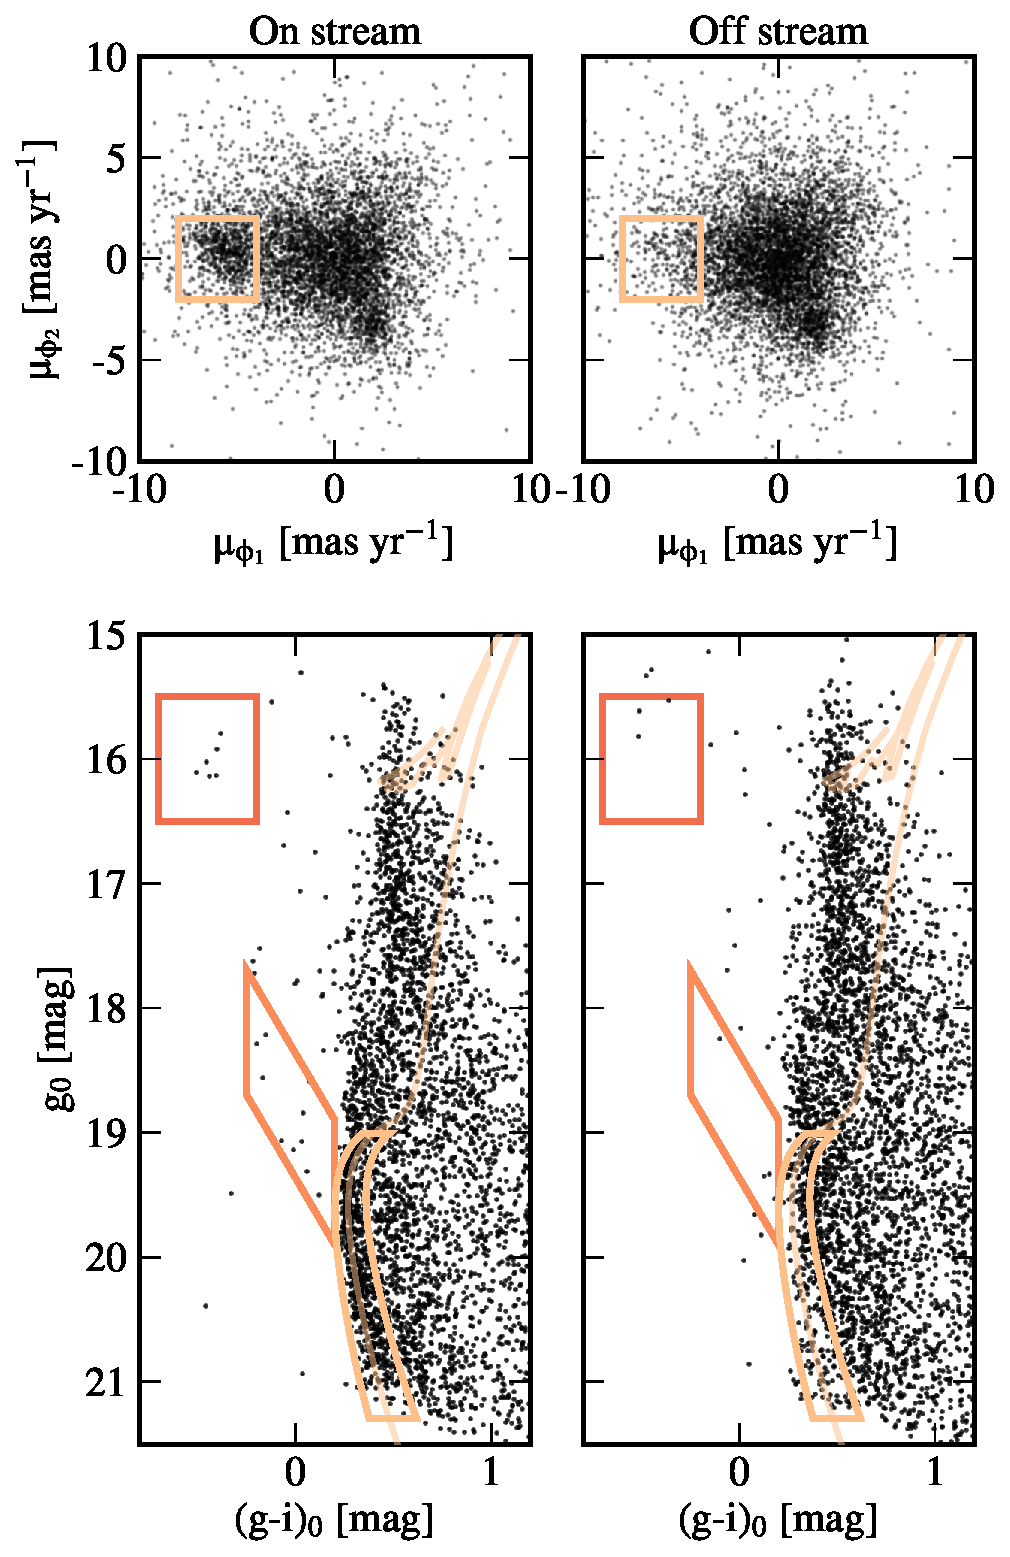
\includegraphics[width=0.95\columnwidth]{selection.pdf}
\end{center}
\caption{
(Top) Proper motions of photometry-selected stars along the Jhelum stream (left) and in a control field (right). 
(Bottom) Similarly, color-magnitude diagrams of stars selected on proper motions.
Photometric and proper-motion selection boxes are shown in light orange.
Jhelum stands out from the Milky Way field population in proper motions as a retrograde stream, and in the color-magnitude diagram where its main sequence is more metal-poor than the field, and is accompanied by blue stragglers (medium orange) and blue horizontal branch stars (dark orange box).
}
\label{fig:properties}
\end{figure}

We query the Gaia DR2 \citep{gdr2} and DES DR1 \citep{abbott2018} catalogs between $-10^\circ<\phi_1<35^\circ$ and $-5^\circ<\phi_2<5^\circ$, and select all sources identified as stars that are brighter than $g_0<23$, while excluding stars with parallaxes larger than $1\,\rm mas$.
DES photometry was dereddened using \citet{sfd} dust maps.
Assuming a constant distance along the stream of 13\,kpc, we correct the whole catalog for the solar reflex motion following \citet{pwb}.

Following these corrections, Jhelum stars becomes readily distinct from the Milky Way field population.
Figure~\ref{fig:properties} shows proper motions (top) and color-magnitude diagram (bottom) for a stream field ($0^\circ<\phi_1<25^\circ$, $0^\circ<\phi_2<1^\circ$, left) and a comparison field ($0^\circ<\phi_1<25^\circ$, $3.5^\circ<|\phi_2|<4^\circ$, right).
In proper motions, Jhelum stands out from the Milky Way as a retrograde stream, and we select likely members between $-8<\mu_{\phi_1,\star}/{\rm mas\,yr^{-1}}<-4$ and $-2<\mu_{\phi_2}/{\rm mas\,yr^{-1}}<2$.
The stream also appears as a prominent overdensity of main sequence stars, which we select following a 12\,Gyr old, metal-poor ($\rm[Fe/H]=-1.5$) MIST isochrone \citep{choi2016} between $19<g_0<21.3$.
Both of these selection regions are shown in light orange in Figure~\ref{fig:properties}.
In the next section, we discuss the spatial distribution of identified Jhelum member stars.


\section{Density structure of Jhelum}
\label{sec:structure}

\begin{figure*}
\begin{center}
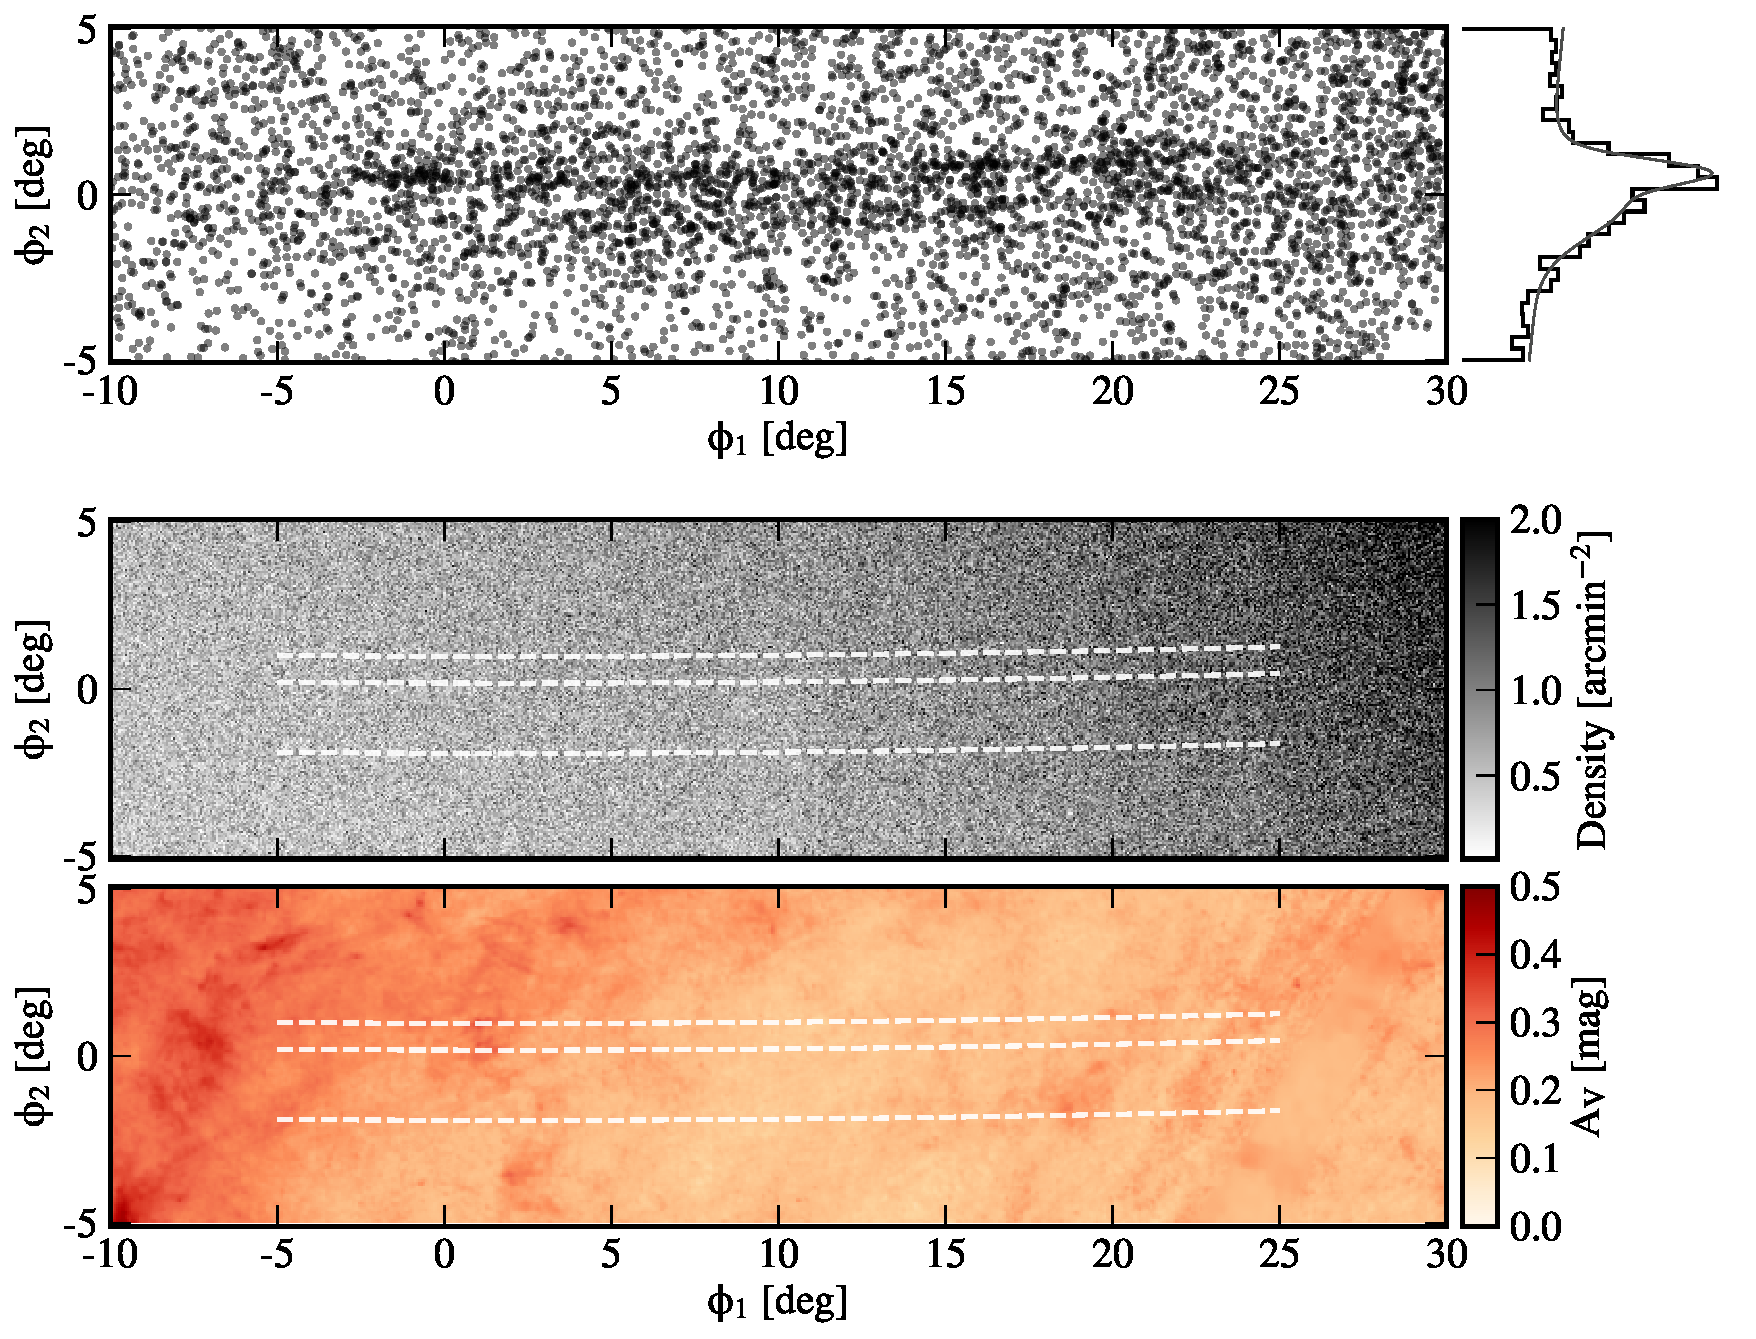
\includegraphics[width=0.9\textwidth]{map.pdf}
\end{center}
\caption{
(Top left) Sky positions of likely Jhelum members in the stream coordinate system reveal for the first time a complex morphology in a cold stream.
Member selection is based on the \gaia\ proper motions and DES photometry, and excludes nearby contaminants using \gaia\ parallaxes.
(Top right) Profile of likely Jhelum members between $-5^\circ<\phi_1<25^\circ$ is asymmetric, with a narrow, dense component at $\phi_2>0^\circ$ and a more diffuse, wide component at $\phi_2<0^\circ$.
This morphology is intrinsic to the stellar stream, as similar signatures are absent from the full stellar density field (middle) and the dust map (bottom).
}
\label{fig:map}
\end{figure*}

Sky positions of Jhelum members selected in Section~\ref{sec:data} are presented in the top left panel of Figure~\ref{fig:map}. 
Although some contamination from the Milky Way field stars remains, the stream stands out as an overdensity between $-5^\circ<\phi_1<25^\circ$, $-1^\circ<\phi_2<1^\circ$.
Despite the increase in the purity of the stream membership, this extent is similar to the initial detection reported by \citet{shipp2018}.
However, the new data reveal unexpected internal structure of the stream: the density of stream members is higher at $\phi_2>0$ than at $\phi_2<0$.
The $\phi_2$ distribution of likely Jhelum members (Figure~\ref{fig:map}, top right) appears bimodal, with a more prominent, narrow component at $\phi_2>0$, and a less prominent, diffuse component peaking at $\phi_2\approx0$.

Surveys such as Gaia and DES have complex selection functions \citep[e.g.,][]{bovy2017}, which can imprint density inhomogeneities in all stellar maps.
To test whether the density structure observed in Jhelum is inherited from a survey strategy, we show a density map of all stars in our input catalog (Gaia crossmatched with DES, and with parallax $\varpi<1\,\rm mas$) in the middle panel of Figure~\ref{fig:map}.
Dashed white lines bracket the two Jhelum components.
The lines are offset from the best-fitting polynomial to the running median of the dense Jhelum component:
\begin{equation}
$\phi_2 = 0.000546 \,\phi_1^2 -0.00217 \,\phi_1 +0.583$
\label{eq:track}
\end{equation}
Whereas there is a large density gradient along the $\phi_1$ direction, as positive $\phi_1$ values correspond to lower galactic latitudes, the overall stellar density changes little across the stream in the $\phi_2$ direction at a fixed $\phi_1$ location.

Density variations observed in streams can also originate from nonuniform dust attenuation \citep[e.g.,][]{ibata2016}.
In that case, the features observed in the stream correlate with a dust map.
Extinction along Jhelum varies between $A_V\sim0.2-0.5$ \citep[Figure~\ref{fig:map}, bottom;][]{sfd}.
The regions of high dust attenuation at $(\phi_1,\phi_2)\approx(1^\circ,0.5^\circ)$ and $(\phi_1,\phi_2)\approx(19^\circ,-2^\circ)$ correspond to regions of reduced Jhelum density, however, there are no global gradients in dust extinction perpendicular to the stream.
Therefore, the transverse variations in Jhelum density are intrinsic to the stream itself.

\begin{figure*}
\begin{center}
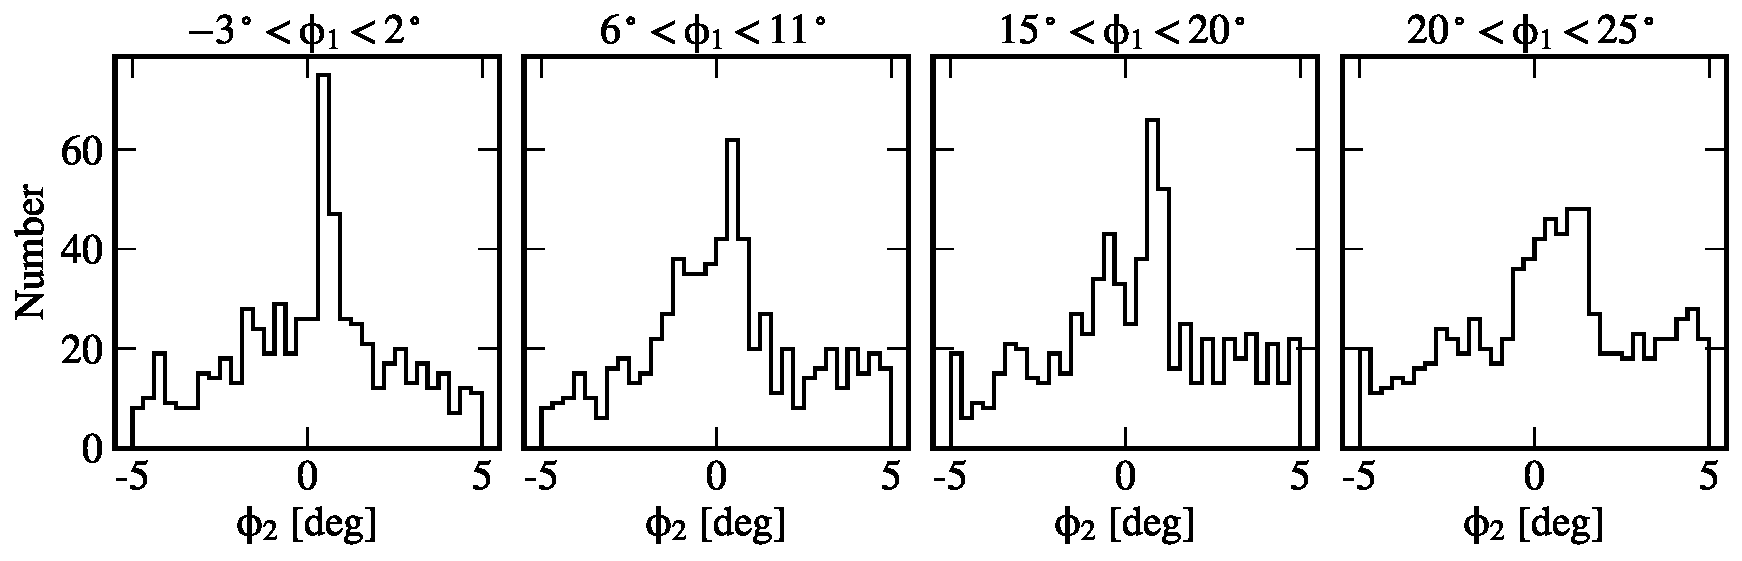
\includegraphics[width=0.9\textwidth]{phi2_histograms.pdf}
\end{center}
\caption{
The profile of likely Jhelum members changes along the stream.
Panels show $5^\circ$ wide regions along the stream, with the location in $\phi_1$ (indicated at the top) growing from left to right.
Between $-3^\circ<\phi_1<2^\circ$, only a narrow component of the stream is present, while in the next $\phi_1$ bin, $6^\circ<\phi_1<11^\circ$, the stream features both the narrow and the wide component.
Further along the stream, $15^\circ<\phi_1<20^\circ$, the stream consists of two narrow components separated by a gap, while at the trailing end, $20^\circ<\phi_1<25^\circ$, the gap vanishes and the stream appears as a single, wide feature.
}
\label{fig:histo}
\end{figure*}

To quantify substructure in the Jhelum stellar stream, we model the $\phi_2$ distribution of likely stream members (Figure~\ref{fig:map}, top right).
We assume a mixture model with two Gaussian components (defined by means $\mu_{1,2}$ and variances $\sigma^2_{1,2}$ for the narrow and wide component, respectively) and a background which is allowed to linearly vary with $\phi_2$ (defined by the gradient $a\rm_{bg}$).
The density model for a given set of parameters $\theta = (\alpha_1, \alpha_2, \alpha_{\rm bg}, \mu_1, \mu_2, \sigma_1, \sigma_2, a_{\rm bg})$ is:
\begin{equation}
\begin{aligned}
p(\phi_2 | \theta) = &\alpha_1 \mathcal{N}(\phi_2 | \mu_1, \sigma_1) + \alpha_2 \mathcal{N}(\phi_2 | \mu_2, \sigma_2) \\
&+\alpha_{\rm bg} (a_{\rm bg}\phi_2 + \mathcal{U}(-5,5))
\label{eq:model}
\end{aligned}
\end{equation}
where $\alpha_{1,2}$ are the fractions of stars in the narrow and wide components, respectively, and $\alpha_{\rm bg} = 1 - \alpha_1 - \alpha_2$ is the fraction of the Milky Way field stars.
We sample the parameter space $\theta$ with an affine invariant Markov Chain Monte Carlo ensemble sampler \citep{emcee}.
The sampler ran with 64 walkers for 4096 steps, the first half of which were discarded as the burn-in, assuming flat priors in normalizations and means, and log-uniform priors for the variances and the background gradient.
The highest-likelihood model (gray line in the top right of Figure~\ref{fig:map}) reproduces well the observed distribution of Jhelum stars.
The amplitudes of both Gaussian components are statistically significant: $\alpha_{1} = 0.102^{+0.008}_{-0.024}$ for the narrow, and $\alpha_{2} = 0.161^{+0.010}_{-0.022}$ for the diffuse component.
Their respective widths are $\sigma_{1} = 0.40^{+0.02}_{-0.06}$\,deg and $\sigma_{2} = 0.94^{+0.04}_{-0.10}$\,deg.
At a distance of 13\,kpc, this corresponds to $w_{1} = 91^{+4}_{-13}$\,pc and $w_{2} = 213^{+8}_{-23}$\,pc, respectively, which is comparable to the widths of globular cluster streams in the Milky Way.

The transverse structure of the Jhelum stream is globally asymmetric, however, there are variations along the stream (see Figure~\ref{fig:map}).
In Figure~\ref{fig:histo} we show the transverse density profiles in four non-overlapping regions.
Splitting the original sample increases the influence of Poisson statistics in the profiles, so we only discuss their features qualitatively.
The left-most panel shows that leading end of the stream ($-3^\circ<\phi_1<2^\circ$) consists of a single, narrow component.
Two components are detected both between $6^\circ<\phi_1<11^\circ$ and between $15^\circ<\phi_1<20^\circ$, however, while the component at smaller $\phi_2$ is wide in the former region (second panel from left), it is narrow in the latter and clearly separated from the narrow component at larger $\phi_2$ (third panel).
At Jhelum's trailing end ($20^\circ<\phi_1<25^\circ$, right-most panel), there is again a single component, but almost twice as wide as that on the leading end.
Curiously, the narrow component visible in the first three panels has an approximately constant width.
This diversity of transverse density profiles along Jhelum underlines the intricacy of its formation history.
In the next section we discuss scenarios which could produce such structures.

\section{Properties of the Jhelum components}
\label{sec:origin}
The Jhelum stellar stream appears to have two spatially distinct components (Figure~\ref{fig:map}).
To uncover their origin, in this section we compare structural and dynamical properties of these components.

% If these components originate from the same progenitor, their stellar populations should be similar and their kinematic profiles should provide insights into dynamical processes that formed them.
% Otherwise, we would expect the components to differ both in stellar population and kinematics.
% To uncover Jhelum's origin, we first compare stellar populations and kinematics in its components, and then explore orbital solutions that fit the stream.

\begin{figure}
\begin{center}
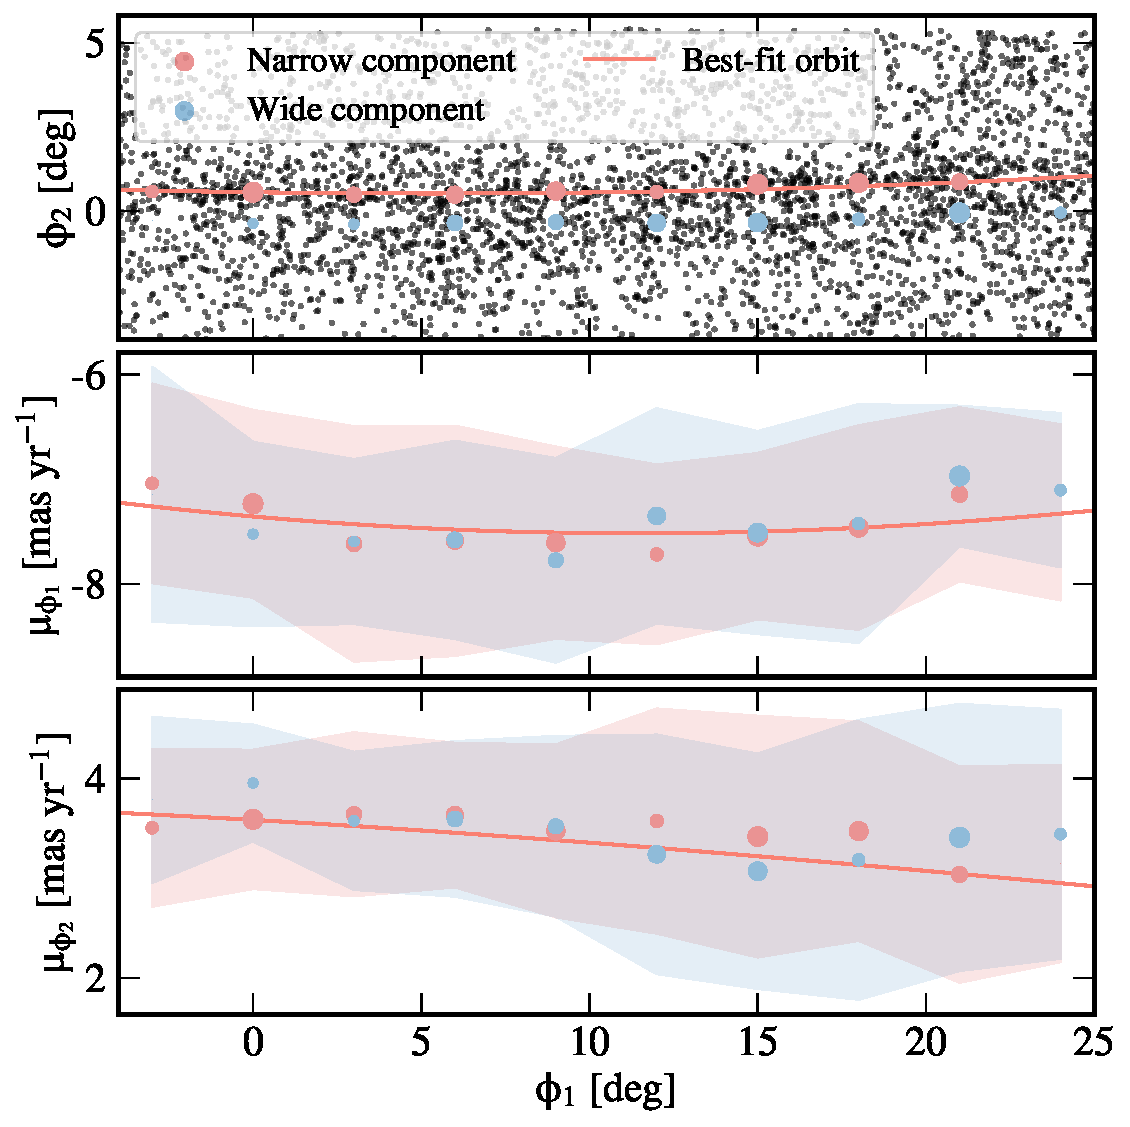
\includegraphics[width=\columnwidth]{components.pdf}
\end{center}
\caption{
On-sky distribution (top) and proper motion profiles (middle, bottom) of the narrow and wide Jhelum components (red and blue points, respectively). 
Spatially offset by $\sim0.9^\circ$, the two Jhelum components have proper motions consistent within uncertainties (shaded area).
The best-fitting orbit in the standard Milky Way potential reproduces the sky and proper motion distribution of the narrow component (thin line).
}
\label{fig:components}
\end{figure}

We first map Jhelum components in the sky and in proper motions.
We spatially define the narrow component as stars within $0.4^\circ$ from the ridgeline (Equation~\ref{eq:track}), and the wide component as stars $0.4^\circ-2^\circ$ below the ridgeline (as shown in Figure~\ref{fig:map}).
For each component, we calculate average properties in $4^\circ$-wide, overlapping bins spaced by $3^\circ$ in the $\phi_1$ direction.
From top to bottom, Figure~\ref{fig:components} shows the running medians of $\phi_2$ positions, $\mu_{\phi_1}$ and $\mu_{\phi_2}$ proper motion components, with red and blue points for the narrow and wide components, respectively.
The size of the point scales with the number of Jhelum stars in the bin, while the shaded area encompasses the median absolute deviation in each component's track.

Both Jhelum components trace a great circle, with their tracks only slightly curving from the $\phi_2=0$ line (Figure~\ref{fig:components}, top).
The components are offset by $\sim0.9^\circ$ in the $\phi_2$ direction, and the offset is constant along the stream.
Despite being spatially offset, the proper motions of the two components are remarkably similar (Figure~\ref{fig:components}, middle and bottom).
% At fixed $\phi_1$, even the proper motion dispersion is comparable between the two components.
The dispersion in proper motions is large ($0.7-1.2\,\rm mas\,yr^{-1}$) and comparable to the observational uncertainties (median for likely Jhelum members is $0.7\rm\, mas\, yr^{-1}$), both of which are much smaller than the typical kinematic offset between the two components ($\lesssim0.3\,\rm mas\,yr^{-1}$).
At the current precision, the Jhelum components are kinematically indistinguishable.

Next, we analyze the stellar population of Jhelum.
Interestingly, blue horizontal branch (BHB) and blue straggler (BS) stars are present in Jhelum, and they are hardly contaminated with field stars (bottom panels of Figure~\ref{fig:properties}).
The ratio of BHB to BS stars can distinguish between massive dwarf galaxy and globular cluster progenitors \citep[e.g.,][]{deason2015}, so we characterize the Jhelum stellar population with the BS to BHB ratio.
We select BHBs at the Jhelum distance with: $-0.7<g-i<-0.2$, $15.5<g<16.5$ (dark orange box in Figure~\ref{fig:properties}) and BSs within the polygon $(g-i,g) = [(0.2,18.9), (0.2, 19.9), (-0.25, 18.7), (-0.25,17.7)]$ (medium orange box).
In the Jhelum footprint (both spatial and proper-motion) there are a total of 31 BSs and 12 BHBs, compared to 12 BS and 2 BHB stars in the control field.
This yields an intrinsic BS to BHB ratio of $N_{BS} / N_{BHB} = 1.9\pm 0.7$, consistent with a $M_V\approx-8$ dwarf galaxy progenitor.
Split between the two components, the ratio becomes $1.7\pm0.9$ and $2.1\pm1.2$ for the narrow and wide component, respectively.
Within uncertainties, the BHB to BS ratio is the same in the two Jhelum components, indicating a common origin.
However, detailed chemical abundances from spectroscopy are required to definitively establish the single-progenitor scenario.

\begin{figure}
\begin{center}
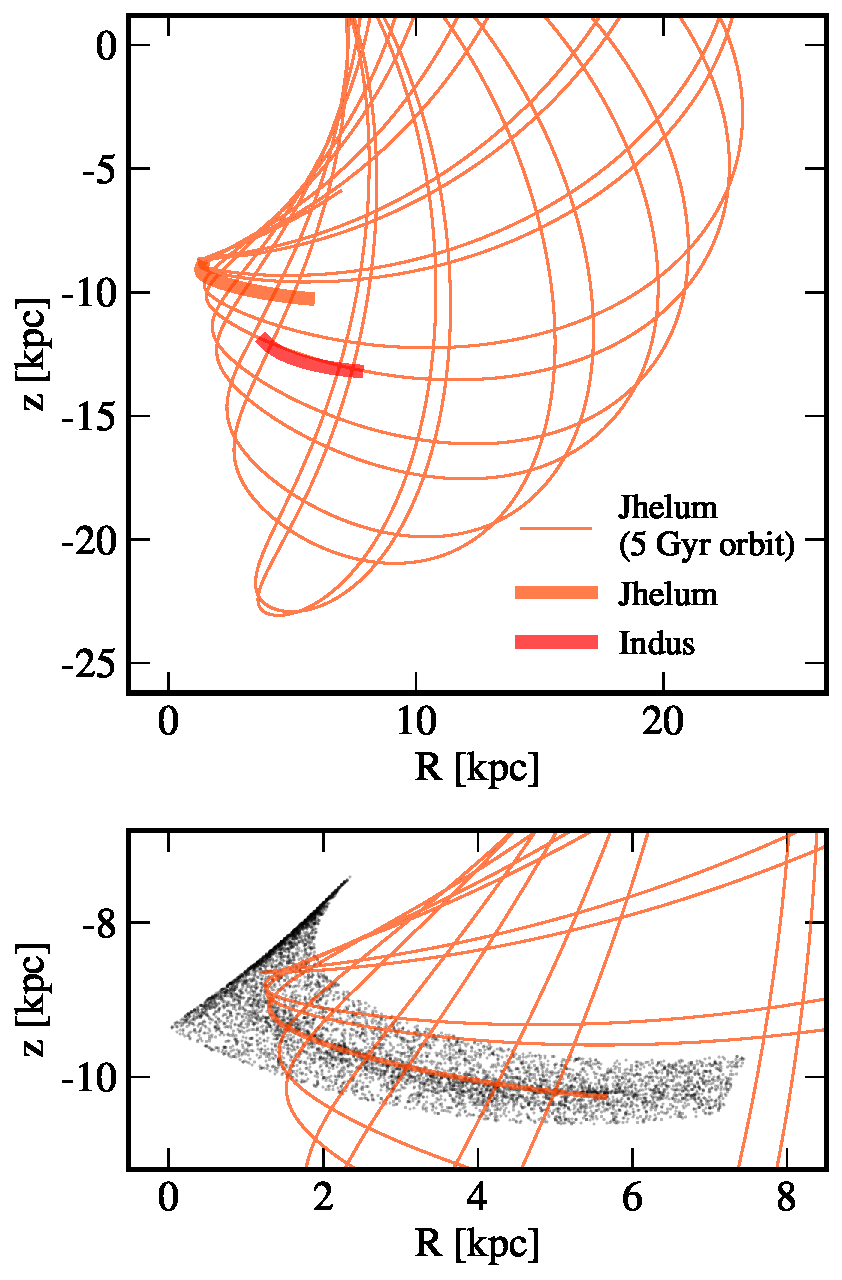
\includegraphics[width=\columnwidth]{orbit_cyl.pdf}
\end{center}
\caption{
Best-fitting orbit of the Jhelum stellar stream in cylindrical Galactocentric coordinates (top).
Thicker portion of the line denotes the observed extent of the stream.
The dense Jhelum component is closer to the Galactic plane than the diffuse component (bottom).
}
\label{fig:galactocentric}
\end{figure}

Finally, we explore whether both of Jhelum components can be accounted for with a simple dynamical model.
Assuming a standard Milky Way potential \citep{gala}, we search for orbits that simultaneously fit the sky distribution of the narrow component, its proper motion profile and that place stream at a constant distance of 13\,kpc.
The best-fitting orbit, shown as a thin line in Figure~\ref{fig:components}, matches well the observed track and proper motion gradients.

In Figure~\ref{fig:galactocentric} we present the Jhelum stream and its best-fitting orbit in cylindrical Galactocentric coordinates.
The thin line traces Jhelum's orbit for the last 5\,Gyr, while the thick line marks the present-day extent of the stream (top panel).
Jhelum orbits between 8 and 24\,kpc, with a period of $\sim300$\,Myr, and is currently just past the pericenter.

- if indus and jhelum are dynamically related, and have a common progenitor, it should have been massive
- this would simultaneously explain the streams' width and the high BS to BHB ratio of a $M_V=-8$ dwarf

The bottom panel of Figure~\ref{fig:galactocentric} zooms in on the stream's current location, and also shows the distribution of likely Jhelum members (assuming the distance gradient from the best-fit orbit).
Jhelum's wide component is $\sim0.5\,\rm kpc$ further from the Galactic plane than its narrow component.
The orbit matches the narrow Jhelum component, but none of the previous orbital wraps pass through the wide component, arguing against the two components being debris of a single progenitor released at subsequent pericentric passages.
In the next section we discuss possible origin scenarios for the transverse structure of the Jhelum stream.


\section{Discussion}
\label{sec:discussion}
The combination of Gaia astrometry and DES photometry allowed us to cleanly select members of the Jhelum stream.
The resulting map reveals Jhelum has two statistically-significant transverse components, separated by $\sim0.9^\circ$.
The two components have similar stellar populations and similar proper motion gradients, which suggests they originate from the same progenitor.
However, in a simple Milky Way potential, the orbit that best-fits the observed distribution of the narrow component fails to simultaneously match the wide component.

Here we discuss possible origin scenarios for the two components of the Jhelum stream:
\begin{itemize}
 \item{\emph{Multiple progenitors:} similar ratio of blue straggler to blue horizontal branch stars indicates the two components have the same stellar population, but there is still room for two distinct progenitors that have similar BS to BHB ratios \citep[e.g., a massive globular cluster and a low-mass dwarf galaxy,][]{deason2015}.
 This hypothesis can be directly tested by measuring chemical abundances in the two components.
 }
 \item{\emph{Kinematic substructure in the progenitor:} disruption of globular clusters initialized in dark matter subhalos leads to non-trivial density structure of the resulting streams \citep[e.g.,][]{penarrubia2017, carlberg2018}.
 In this scenario, the wide component of Jhelum would be stars stripped while the globular cluster was still in the subhalo \citep[similar to the recently reported GD-1 cocoon,][]{malhan2019}, while the narrow component would be stars more recently released directly in the Milky Way gravitational potential.
 The velocity dispersion in each component should reflect their local environment prior to the formation of the stream \citep[e.g.,][]{fardal2015}.
 Precise measurements of either proper motions or radial velocities can test whether the wide component is indeed kinematically hotter than the narrow one.
 }
 \item{\emph{Fold caustic:} tidal debris distributed in a plane, but viewed almost edge-on, could feature the bimodal density profile observed in Jhelum.
 Two-dimensional shells are commonly observed \citep[e.g.,][]{tal2009,kadofong2018}, however, their densest part, unlike Jhelum's, is at the largest galactocentric radius.
 A more general fold caustic of a fully phase-mixed distribution is still allowed \citep[e.g.,][]{tremaine1999}, in which case the velocity dispersion in the dense component of Jhelum should be higher than in its diffuse part.
 Precise kinematics will test this formation pathway as well.
 }
 \item{\emph{Precession of the orbital plane:} streams orbiting in non-spherical potentials widen because their orbits precess \citep[e.g.,][]{erkal2016, dehnen2018}.
 Jhelum's orbit is significantly affected by the Milky Way disk, so its extended structure may be attributed to orbital precession.
 This effect is not captured in simple streakline models of streams, so more detailed, $N$-body modeling of Jhelum is required.
 }
 \item{\emph{Chaos:} streams formed close to a resonant orbit often have low surface-brightness envelopes \citep[e.g.,][]{pw2016}.
 In a simple gravitational potential, Jhelum's orbit is regular (see Figure~\ref{fig:galactocentric}).
 However, a chaotic orbit may still be possible if the adopted potential is very different from the true one.
 }
 \item{\emph{Time-dependent perturbations:} massive, dynamical perturbers such as the rotating bar or Large Magellanic Cloud (LMC) can affect the structure of stellar streams \citep[e.g.,][]{pearson2017, erkal2019}.
 Since Jhelum is orbiting in the inner Galaxy, the LMC is likely not a major perturber (their closest approach was $\gtrsim30$\,kpc).
 However, Jhelum comes within $\sim8\,$kpc from the Galactic center, where the bar may influence even streams on retrograde orbits.
 }
\end{itemize}

All these formation scenarios merit further investigation, but we prefer solutions where Jhelum is still a coherent tidal structure on a largely unperturbed orbit.
Our best-fit orbit for Jhelum simultaneously (and independently) matches the Indus stream, suggesting that only minor effects are allowed from the bar, chaos or LMC.
Both streams are still coherent, so this argues against the fold caustic interpretation for Jhelum's vertical structure.
The remaining scenarios can be distinguished with a combination of spectroscopic data and more detailed dynamical modeling.
Chemical abundances will determine whether both Jhelum components originate from the same progenitor.
In the case of a single progenitor, confronting the theoretical and observed radial velocities in the two Jhelum components will differentiate between them originating from different substructures within the progenitor or being precessing debris.

- streams rich in information
- dynamics within the stream, multiple linked
- long very informative -- good for global scale
- structure within streams -- tell about smaller scales

\acknowledgements

Kathryn, Ray, Scott

This project was developed in part at the 2018 \acronym{NYC} \gaia\ \acronym{DR2} Workshop at the Center for Computational Astrophysics of the Flatiron Institute in New York City in 2018 April.

This work has made use of data from the European Space Agency (\acronym{ESA}) mission \gaia\ (\url{https://www.cosmos.esa.int/gaia}), processed by the \gaia\ Data Processing and Analysis Consortium (\acronym{DPAC}, \url{https://www.cosmos.esa.int/web/gaia/dpac/consortium}). Funding for the \acronym{DPAC} has been provided by national institutions, in particular the institutions participating in the \gaia\ Multilateral Agreement.

% This project used public archival data from the Dark Energy Survey (DES). Funding for the DES Projects has been provided by the U.S. Department of Energy, the U.S. National Science Foundation, the Ministry of Science and Education of Spain, the Science and Technology FacilitiesCouncil of the United Kingdom, the Higher Education Funding Council for England, the National Center for Supercomputing Applications at the University of Illinois at Urbana-Champaign, the Kavli Institute of Cosmological Physics at the University of Chicago, the Center for Cosmology and Astro-Particle Physics at the Ohio State University, the Mitchell Institute for Fundamental Physics and Astronomy at Texas A\&M University, Financiadora de Estudos e Projetos, Funda{\c c}{\~a}o Carlos Chagas Filho de Amparo {\`a} Pesquisa do Estado do Rio de Janeiro, Conselho Nacional de Desenvolvimento Cient{\'i}fico e Tecnol{\'o}gico and the Minist{\'e}rio da Ci{\^e}ncia, Tecnologia e Inova{\c c}{\~a}o, the Deutsche Forschungsgemeinschaft, and the Collaborating Institutions in the Dark Energy Survey.
% 
% The Collaborating Institutions are Argonne National Laboratory, the University of California at Santa Cruz, the University of Cambridge, Centro de Investigaciones Energ{\'e}ticas, Medioambientales y Tecnol{\'o}gicas-Madrid, the University of Chicago, University College London, the DES-Brazil Consortium, the University of Edinburgh, the Eidgen{\"o}ssische Technische Hochschule (ETH) Z{\"u}rich,  Fermi National Accelerator Laboratory, the University of Illinois at Urbana-Champaign, the Institut de Ci{\`e}ncies de l'Espai (IEEC/CSIC), the Institut de F{\'i}sica d'Altes Energies, Lawrence Berkeley National Laboratory, the Ludwig-Maximilians Universit{\"a}t M{\"u}nchen and the associated Excellence Cluster Universe, the University of Michigan, the National Optical Astronomy Observatory, the University of Nottingham, The Ohio State University, the OzDES Membership Consortium, the University of Pennsylvania, the University of Portsmouth, SLAC National Accelerator Laboratory, Stanford University, the University of Sussex, and Texas A\&M University.
%
% Based in part on observations at Cerro Tololo Inter-American Observatory, National Optical Astronomy Observatory, which is operated by the Association of Universities for Research in Astronomy (AURA) under a cooperative agreement with the National Science Foundation.

\appendix
% \section{Jhelum rotation matrix}
% \begin{widetext}
\begin{equation*}
\begin{bmatrix}
\cos(\phi_1)\cos(\phi_2)\\
\sin(\phi_1)\cos(\phi_2)\\
\sin(\phi_2)\\
\end{bmatrix}
 = 
\begin{bmatrix}
0.6173151074 & -0.0093826715 & -0.7866600433 \\ 
-0.0151801852 & -0.9998847743 & 0.0000135163 \\ 
-0.7865695266 & 0.0119333013 & -0.6173864075 \\ 

\end{bmatrix}
\begin{bmatrix}
\cos(\alpha)\cos(\delta)\\
\sin(\alpha)\cos(\delta)\\
\sin(\delta)\\
\end{bmatrix}
\label{eq:rotmat}
\end{equation*}
% \end{widetext}

\bibliographystyle{aasjournal}
\bibliography{jhelum}



\end{document}

